\section{INTRODUCTION}\label{sec:1introduction}

Sleep plays a vital role in good health and well-being throughout a person's life. Lacking of sleep or having poor sleep can lead to
serious, sometimes life-threatening, health problems~\cite{lallukka2016contribution}. The quality of sleep depends on many factors,
including the sleeping environment such as the light intensity and the ambient temperature, the user's breath, the sleeping posture, and
the bedtime routine. By capturing information of these factors, sleep monitoring can help one to assess and understand his sleeping
pattern, and improving the sleep efficiency by providing feedback on how the change of the sleeping environment and behavior affect the
sleeping quality.

Traditionally, sleep monitoring had to be done in a clinic environment using dedicated medical equipment like electroencephalography (EEG), electrocardiography (ECG) and electromyography (EMG).  Modern mobile devices such as smartphones and smartwatches offer a new way for sleep monitoring. By utilizing the sensors integrated on the mobile device, we can track certain physical activities such as body movement or snore, and use the tracked information to detect the sleep pattern~\cite{zeo,Jawbone,SleepAndroid,fitbit,gu2016sleep}. Such an approach is known as \emph{actigraphy}~\cite{Actigraphy,ancoli2003role}. Using mobile devices to monitor sleep has a number of advantages over a clinic solution, including being lower cost and non-invasive, and can be performed at home on an on-going basis.

%There is a common way to monitor sleep through a polysomnography (PSG) \cite{Polysomnography}. Polysomnography, including
%electroencephalography (EEG), electrocardiography (ECG), electromyography (EMG), chest and abdominal breathing tension map, and so on more
%than 10 channels of physiological signals, mainly for sleep and dream studies and the diagnosis of depression and sleep apnea syndrome.
%However, PSG-based sleep quality measurement is usually limited to clinical settings. Another approach is actigraphy \cite{Actigraphy},
%which utilizes rich sensors on wearable devices to monitor some certain physical activities such as body movement or snore
%\cite{zeo,Jawbone,SleepAndroid,fitbit,gu2016sleep}, to detect sleep pattern. With the advantages of low cost, non-invasive and simple
%operations, wearable devices such as smartwatch becomes increasing interested by the public recent years. Recent years, many apps have %been developed on the market \cite{,Jawbone,fitbit}. However, they provide few details about how the systems conclude the sleep report. In %fact, the sleep related events usually imply more elaborate details about the body and health.  Another negative effect for the absence of sleep %details is that it makes the consumers confused about the


However, existing mobile-based sleep monitoring applications fail to fully exploit the sensors provided by modern mobile devices. As a
result, current mobile-based sleep monitoring system typically only provide superficial information such as the duration of deep and
shallow sleep. Without further detailed information of the environment and activities across sleep stages, these applications offer little
help in understanding the causes of poor sleep. To unlock the potential of mobile-based sleep monitoring, we need to find ways to take full
advantage of the rich sensor data provided by modern mobile devices.


The work presented by Gu \etal~\cite{gu2016sleep} is among the first attempts in this direction
\cite{lawson2013validating,bauer2012shuteye,min2014toss,al2014classifying}. Their work exploits smartphone sensors to detect physical and acoustical activities happened during sleep. While promising, this approach requires placing the smartphone next to the user's head and
ensuring the phone remains stationary throughout the sleeping process. However, this requirement often cannot be satisfied and many users
do not want to place the mobile phone too close to the body due to health risk concerns~\cite{StepHealth,Quorasleep}.

\begin{figure}[!t]
\centering
\setlength{\belowcaptionskip}{-13pt}
      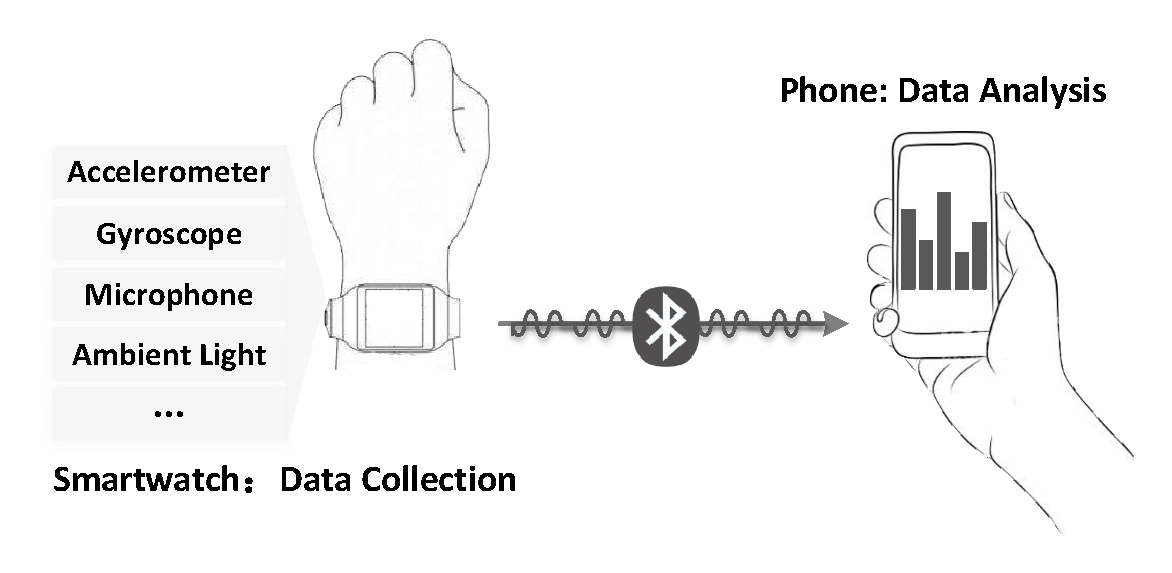
\includegraphics[width=0.87\linewidth]{Figures/datacollect.pdf}
  \caption{{\systemname} detects a wide range of sleep-related activities and events using a smartwatch.}\label{fig:datacollect}
\end{figure}

This paper presents a better approach. Instead of using smartphones and relying on strict, unrealistic assumptions, we exploit the rich
sensor data provided by smartwatches to track a wider range of sleep-related activities. The advantages of using a smartwatch are that
many users are willing to wear the device throughout the night, thus the device can remain relatively close to the user over the duration
of sleep.  The smartwatch also allows us to collect a richer set of information. The collected information can then be used to monitor a
wider range of sleep-related events. While there are prior works on sleep monitoring based on smartwathes
\cite{pombo2016ubisleep,shelgikar2016sleep,haescher2015anomaly,borazio2012combining}, these approaches only gather coarse-grained
information and often rely on specialize devices such as pressure mattresses or image acquisition equipment. In this work, we demonstrate
that, for the first time, smartwatches enable us to collect an extensive set of sleep-related events -- many of which are not supported in
prior work. Having a more comprehensive set of sleep-related events and activities will thus enable users to gain a deeper understanding of
their sleep patterns and the causes of poor sleep.

%sleeping process. This changing nature can introduce tremendous noise to the sensor data, making it difficult to associate the sensor data
%with sleep-related physical and acoustical activities. Overcome this challenge requires


%In this paper, we present {\systemname} - the first deep understanding system about the smartwatch based sleep monitoring. In line with common actigraphy system, the rich sensing information by sensors (accelerometer, gyroscope, microphone and ambient light sensor) are transmitted to the sever (smartphone or computer, etc) and used to detect the sleep related events. Unlike existing approaches, we are the first time to analysis the comprehensive information of the sleep events and verify their dependabilities. Consequently, our system can not only report the ultimate sleep quality, but also more details about different sleep events. The key insight behind {\systemname} is that the sleep quality is highly correlated with the sleep posture, acoustic event and even the illumination condition. We present straightforward algorithms to detect multiple effects during sleep. Then we incorporate the detected events, deduce the user's sleep stages and sleep quality.
%
%Specifically,  {\systemname} can monitor the user's sleep posture and habits, which is an indispensable factor of determining sleep quality and is heavily used in performing medical diagnoses \cite{oksenberg1998effect}. For example, the supine body position will aggravate the breath abnormalities and cause the sleep disorders. An effective posture detection and timely posture change can improve obstructive sleep apnea. In addition, the hand position \cite{AskMetaFilter} during sleep discloses some potential health problems and some improper hand position will bring bad results. For instance,  the hand position on the abdomen or head may indicate its uncomfortable state, while the person is usually not aware of that case; and when the hand is put on the chest, the person is easy to have a nightmare because of the long-term oppression on the heart. Thus to analyze the user's sleep quality effectively, we present three algorithms to detect four common sleep postures, the posture transitions and the hand position during sleep.
%
%{\systemname} can also detect different sound events during sleep, which is another most important indicators of sleep quality. The snoring, coughing and somniloquy can suggest user's sleep quality and physical health. For example, snoring is one of the possible symptoms of cerebral infarction patients. Different from traditional parameters based acoustic classification algorithm \cite{gu2016sleep}, we exploit the inherent characteristics of different acoustic events and design a lightweight algorithm for effective classification. Furthermore, {\systemname} analyzes the illumination conditions, detects the micro body movements such as limb trembling and head movement, etc. Finally, {\systemname} integrates those events to infer the user's sleep stages on the framework of Hidden Markov Model, and estimate the sleep quality based on the detected sleep stage sequence.

%\begin{figure*}[!thbp]
%\centering
%      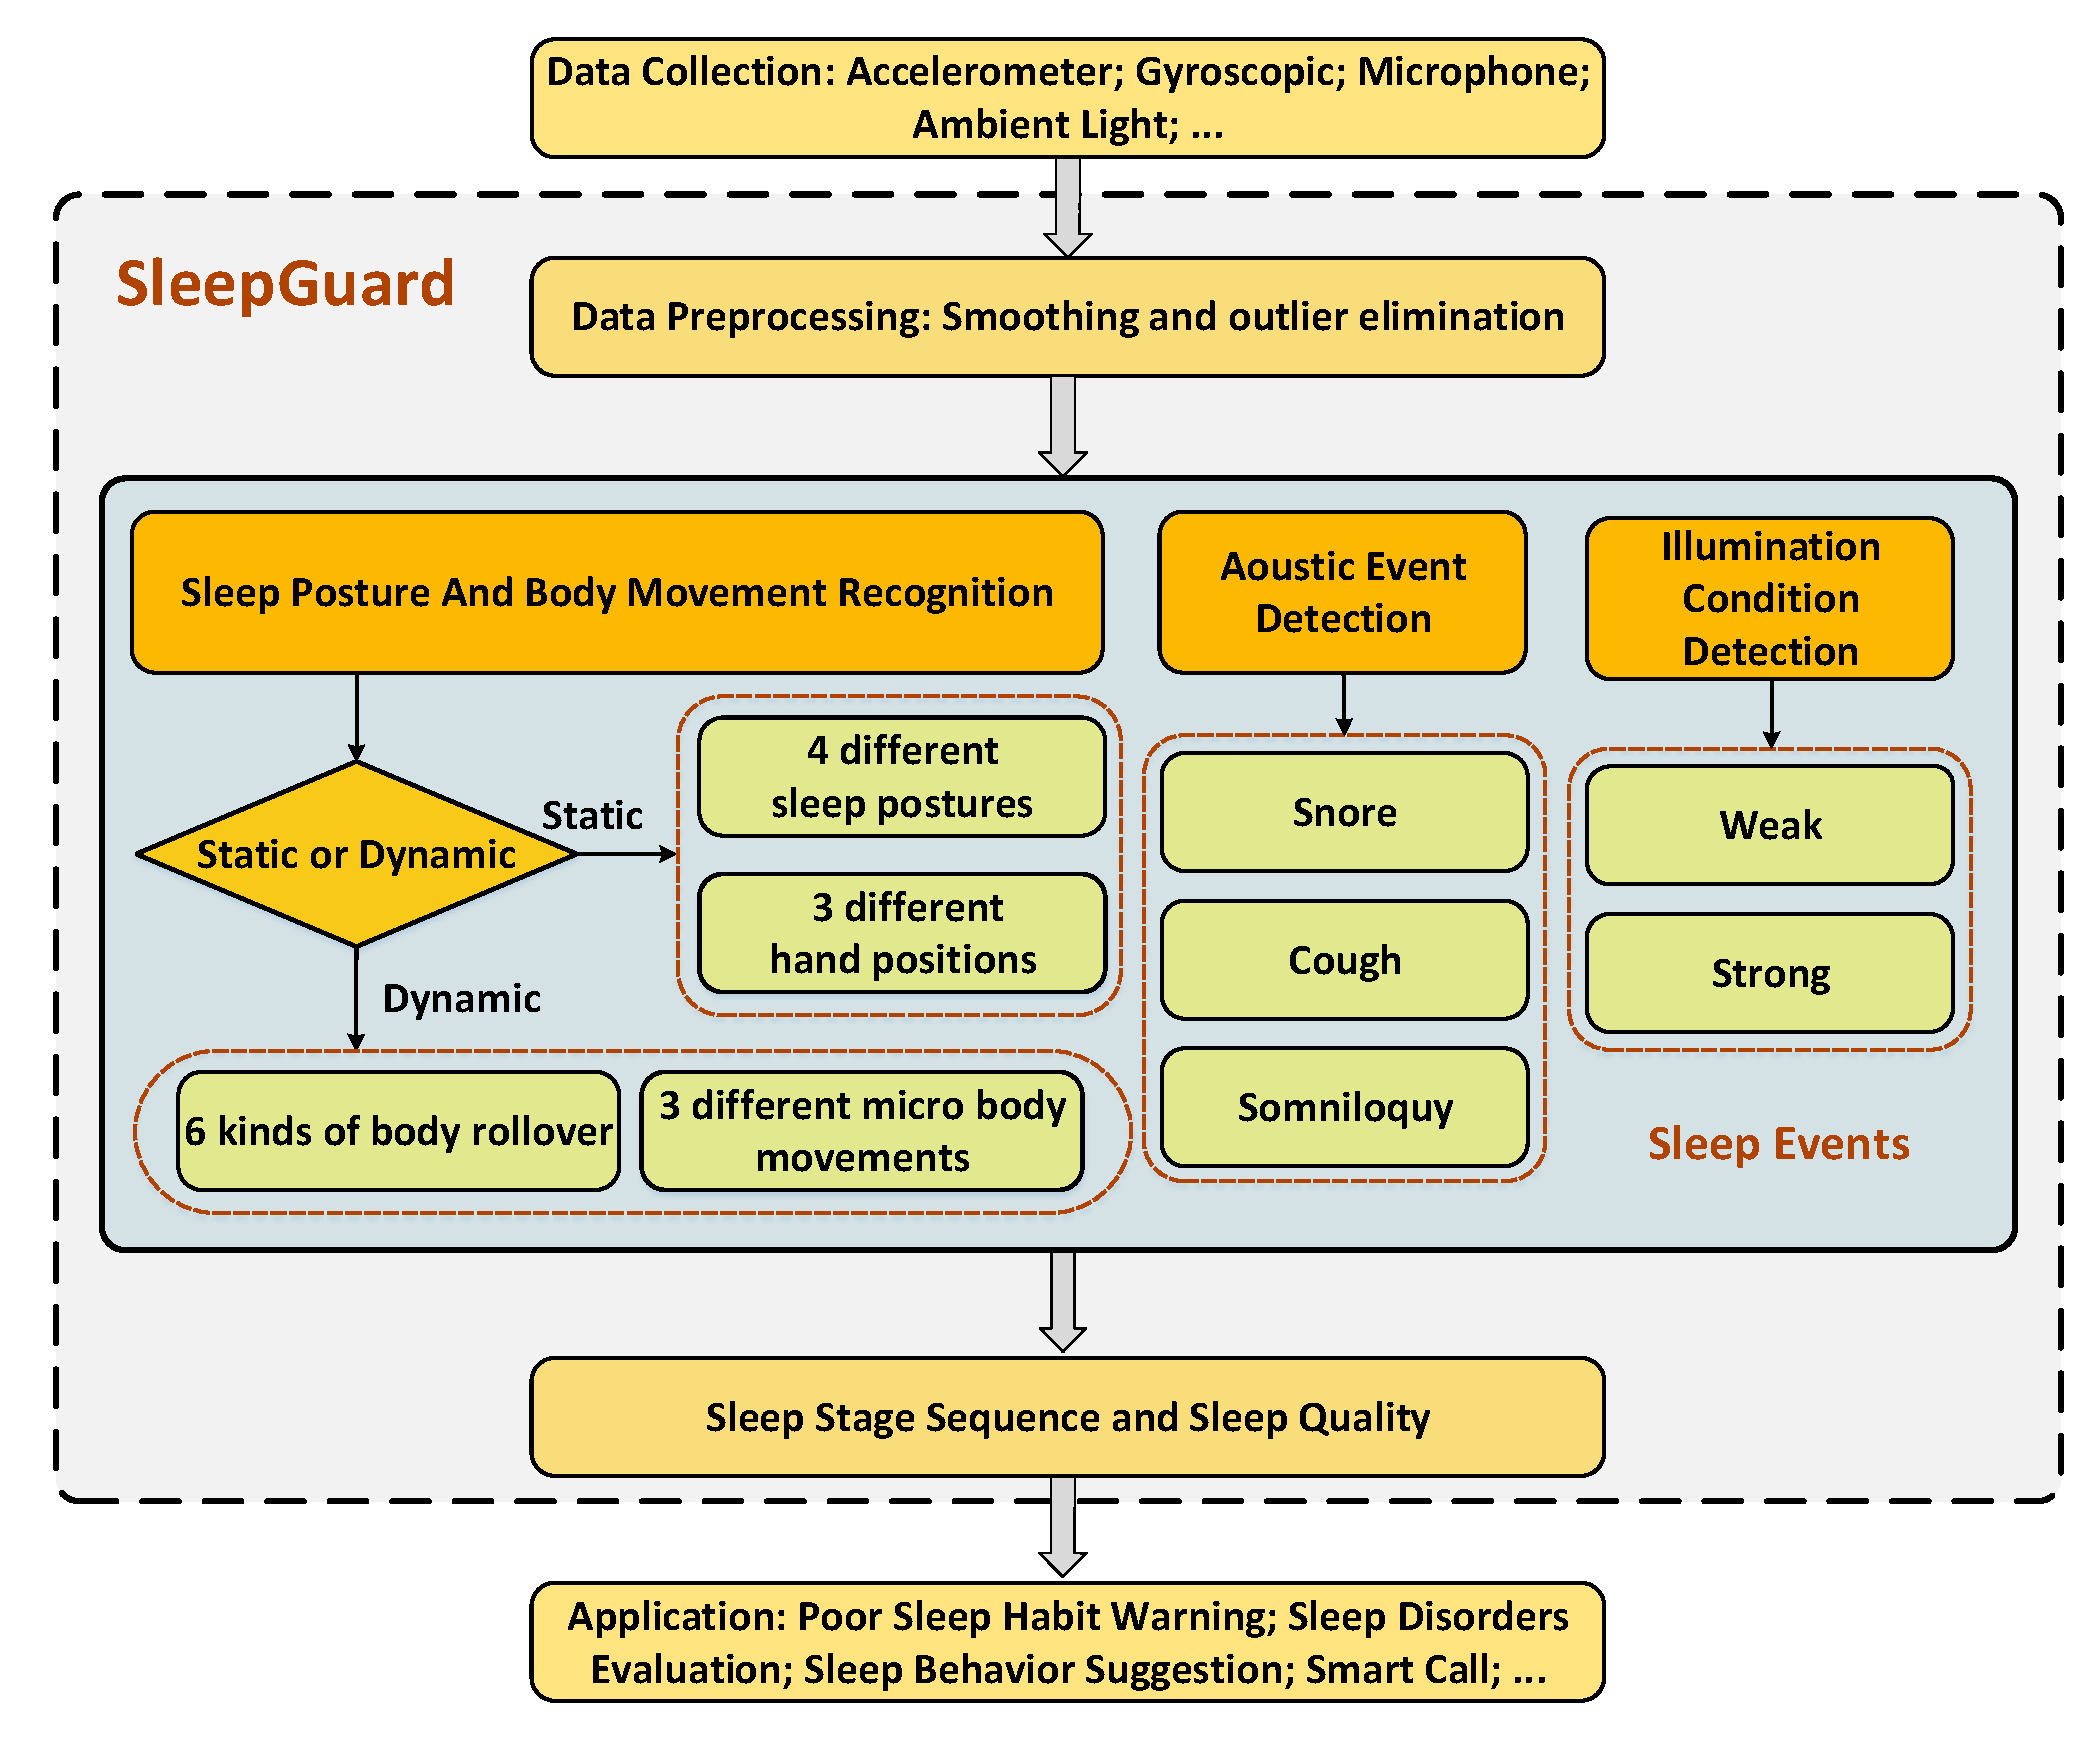
\includegraphics[width=0.57\linewidth]{Figures/SystemFlow.pdf}
%  \caption{System overview of {\systemname}.}\label{fig:overview}
%\end{figure*}

In this paper, we present \systemname, the first smartwatch-based monitoring system that can track a wide range of sleep-related
activities. \systemname gathers sleep-related activities by utilizing the commonly available sensors on smartwatches: the accelerometer,
gyroscope, microphone and ambient light sensor, etc. It then uses the tracked information to infer the user's sleep posture and habits --
thing like changes of body and hand positions, as well as sound events due to e.g. snoring or coughing.  Collecting these data can help a
user to gain a deep understanding of his/her sleeping pattern and quality, and to find ways to improve sleep.

However, translating the collected senor data to these sleeping events is non-trivial due to the changing nature of smartwatches during
sleep. To overcome these challenges, we develop a set of new methods and analysis, specifically targeting portable mobile devices.  The key
insight behinds {\systemname} is that the sleep quality is strongly correlated to the sleep posture, acoustic events and the illumination
condition \cite{shelgikar2016sleep}. By exploiting the unique characteristics of sensory data produced by different sleep activities, we develop a series of novel algorithms to correlate the sensory data to sleep events. We then design a model to incorporate the detected events to
infer the user's sleep stages and sleep quality.

We evaluate our approach by applying it to ten users over two weeks period. The experimental results show that {\systemname} is  effective and accurate in capturing sleep-related activities. For body posture classification, body rollover recognition, hand position identification and  acoustic events detection,  it achieves least accuracies of 98\%,  90\%,  87\% and  96.9\%, respectively. These results show that {\systemname}  is superior to existing actigraphy-based applications.

Our main contributions are:

\begin{itemize}[itemsep=1mm,nolistsep]

\item We present a novel sleep monitoring system based on smartwatch sensor information. Our system captures a wider range of sleeping
    activities that none of the current mobile-based sleep monitoring solutions can offer.

\item We design a set of new algorithms and analysis to effectively exploit the smartwatch sensor data to detect sleep-related
    activities. These include body postures, body rollovers, hand positions, micro body movements and acoustical events.

\item The experimental results suggest that our prototype system, \systemname, is highly effective in capturing sleep-related events.

\end{itemize}



%This work makes the following specific contributions:
%
%
%%The design of our system involves the following contributions:
%\begin{itemize}
%  \item We present the first deep understanding system about the smartwatch based sleep monitoring. The system integrates the rich sensing data to analyze the user's detailed sleep events, and then estimate the sleep stages and quality.
%  \item Based on a serious of key observations during sleep, we design three novel algorithms to effectively detect the body posture, posture transition and hand position without resorting to any extra devices.
%  \item By utilizing the underlying characteristics of different acoustic events, we propose an innovative algorithm to classify different sounds during sleep. The algorithm can be easily extended for other sound classifications.
%  \item We prototype {\systemname} on HuaWei smartwatch and test 10 users for two weeks. The extensive results show that smartwatch based sleep monitoring can provide a relatively high accuracy, thus give a reliable advice about the sleep quality.
%\end{itemize}


%\begin{figure}[!t]
%\centering
%\begin{minipage}[t]{0.575\linewidth}\centering
%      \includegraphics[width=9cm,height=4cm]{Figures/big.pdf}
%  \caption{(a), (b) and (c) are three strokes composing the Chinese character "Big"; (d) pen moves from the first stroke's end point to the second stroke's start point.}\label{fig:big}
%\end{minipage}
%\hspace{1pt}
%\begin{minipage}[t]{0.405\linewidth}\centering
%      \includegraphics[width=5cm,height=4cm]{Figures/segment.pdf}
%  \caption{Pen movement process during a meaningless stroke. }\label{fig:segment}
%\end{minipage}
%\end{figure}
%
%\begin{figure}[!t]
%%\centering
%\begin{minipage}[t]{0.33\linewidth}\centering
%      \includegraphics[width=1\linewidth]{Figures/3Dsegmenta.pdf}
%  \caption{The 3D location view of the brush pen and antennas.}\label{fig:3Dsegmenta}
%\end{minipage}
%\hspace{2pt}
%\begin{minipage}[t]{0.3\linewidth}\centering
%      \includegraphics[width=3.5cm,height=3.5cm]{Figures/3Dsegmentb.pdf}
%  \caption{Obtain the value of distance $h_1$.}\label{fig:3Dsegmentb}
%\end{minipage}
%\hspace{2pt}
%\begin{minipage}[t]{0.3\linewidth}\centering
%      \includegraphics[width=3.5cm,height=3.5cm]{Figures/3Dsegmentc.pdf}
%  \caption{Obtain the value of distance $h_2$.}\label{fig:3Dsegmentc}
%\end{minipage}
%\end{figure}
